% Chapter Template

\chapter{Conclusions and Future Work} % Main chapter title %% EXTRACT RESULTS SECTION FROM HERE TO NEW CHAPTER

\label{Chapter6} % Change X to a consecutive number; for referencing this chapter elsewhere, use \ref{ChapterX}

%----------------------------------------------------------------------------------------
%	SECTION 1   % TARGET 1500 WORDS IN THIS CHAPTER
%----------------------------------------------------------------------------------------

\section{Overview}
The MEGAphone accessible interface project was fully realised on the 8th of November, 2020.
This chapter provides concluding remarks on the deliverables of the project including the research questions and contributions of the author.
A discussion on aspects where the project might benefit from future research is also addressed in this final chapter.

%----------------------------------------------------------------------------------------
%	SECTION 2
%----------------------------------------------------------------------------------------

\section{MEGAphone Chassis/Case First Revision}
This section reviews how the research questions were answered and recounts the contributions made by the author.

% %-----------------------------------
% %	SUBSECTION 1
% %-----------------------------------
\subsection{Research Questions}

This thesis has answered the following research questions in the preceding chapters:
\begin{enumerate}
    \item What is the relationship between Digital Sovereignty and Universal Design?
        \begin{enumerate}
        \item[-] Chapter \ref{Chapter1} introduced these concepts and their characteristics.
        \item[-] Chapter \ref{Chapter2} set out to establish what each of these concepts meant along with their importance in this project.
        \item[-] Chapter \ref{Chapter4} took those concepts and applied them to a real tangible design, drawing commonality between these concepts along the way.
        \end{enumerate} 
    \item Why is Universal Design important in the design of products today?
        \begin{enumerate}
        \item[-] Chapter \ref{History} established why UD is important, as the concept attempts to normalise accessible design practices so that people with a disability or of old age can be better included in the products of today.
        \item[-] Chapter \ref{Chapter4} applied that concept, highlighting the importance of such features and how not only those with a disability, but also abled bodied people can benefit. 
        \end{enumerate}
    \item Why is Digital Sovereignty important in the design of electronic products today?
        \begin{enumerate}
        \item[-] Chapter \ref{MEGAphone} covers the MEGAphone mobile device and how users can benefit from an open and secure platform.
        \item[-] Chapter \ref{KiCAD} explained how considering open-source software in the development of the project can make it easier for users to modify aspects of the product after the fact.
        \item[-] Chapter \ref{Chapter4} presented examples of DS in practice, such as the solar cell feature in section \ref{Solar Cells}, which provides users with an alternative way to charge their device, making them no longer solely dependent on working energy infrastructure.
        \end{enumerate} 
    \item How can the seven design principles be used in the design of the MEGAphone case to support those with disabilities?
        \begin{enumerate}
        \item[-] Chapter \ref{Motivation} introduces the seven design principles as a tool to measure the accessibility of a product.
        \item[-] Chapter \ref{Seven Principles} goes into detail on these principles and briefly explains the characteristics of each design principle.
        \item[-] Chapter \ref{Chapter4} provides evidence of the seven design principles in practice, highlighting how they apply to each design feature.
        \end{enumerate} 
    \item How can the 'Right to Repair' philosophy be used in support of the universally designed MEGAphone case?
        \begin{enumerate}
        \item[-] Chapter \ref{Planned Obsolescence} discussed how planned obsolescence works in favour of the manufacturer and against the user and the freedoms that the user gives up as a result.
        \item[-] Chapter \ref{Chapter4} provides evidence as to how this philosophy can support the project, such as making the internal components easy to access to those who desire access (view section \ref{Threaded}), while not sacrificing safety for those who don't, as per the UD concept.
        \end{enumerate} 
    \item What are the effects of COVID-19 on Digital Sovereignty, Universal Design and the MEGAphone project?
        \begin{enumerate}
        \item[-] Chapter \ref{Objectives} and chapter \ref{First Revision} explains that this pandemic disrupted the iterative design process as focus groups consisting of people with disabilities for design feedback was abandoned due to the health risks of the virus.
        \item[-] Chapter \ref{Capability} looks at the effects of COVID-19 related to capability maintenance, what a device means to be 'sovereign' and what this potentially means for people with a disability.
        \end{enumerate} 
\end{enumerate}

% %-----------------------------------
% %	SUBSECTION 2
% %-----------------------------------
\subsection{Contributions to the Field}

The author's key contributions to the field, recounted in detail, are:
\begin{enumerate}
    \item An examination of the relationship between Digital Sovereignty and Universal Design.
        \begin{enumerate}
        \item[-] As recounted in the previous subsection, this thesis provides a comprehensive examination of the UD and DS concepts and the relationship that they share.
        \end{enumerate} 
    \item Analysis of the existing MEGAphone PCB design from the perspective of UD.
        \begin{enumerate}
        \item[-] This project delivers three new PCB designs, to interface with the existing PCB, in order to better adapt it to the principles of UD.
        \end{enumerate} 
    \item The creation through iteration of a UD housing for the MEGAphone PCB.
        \begin{enumerate}
        \item[-] Chapter \ref{Chapter4} provides a comprehensive review of the UD housing for the MEGAphone project, including evidence of an iterative design process (view section \ref{First Print} and section \ref{CAD Models}).
        \item[-] Chapter \ref{Chapter5} further supports this by providing the CAD work for a future 3D-print of the project.
        \end{enumerate} 
    \item The improvement of the MEGAphone device layout to improve its UD properties.
        \begin{enumerate}
        \item[-] Evidence of this during the project is presented in the form of smaller external PCBs that serve to interface with the main PCB for the sake of delivering an accessible prototype (view chapter \ref{PCBs}), thereby avoiding a costly and time-consuming redesign of the MEGAphone.
        \item[-] The implementation of the 'EZ access keys' provides the MEGAphone device with a useful alternative method of use which supports UD principles {view chapter \ref{EZkeys}}.
        \item[-] Accompanying the 'EZ access keys' is the adaptation of large rocker switches which make controlling power to various modules of the MEGAphone far easier than previously possible (view chapter \ref{Rocker Switches}).
        \item[-] Hardware-implemented 'software' features transparent to the MEGA65 OS provide users with an alternative method of interacting with the keyboard (view chapter \ref{Software Access}), through the use of a Jellybean switch.
        \end{enumerate} 
    \item The design of practical modifications to the MEGAphone PCB design that allows the majority of the UD improvements to be realised, without requiring a complete and costly redesign of the MEGAphone PCB.
        \begin{enumerate}
        \item[-] This links closely with the previous contribution where these practical modifications are realised as supporting PCBs which interface with the main PCB.
        \end{enumerate} 
    \item The proposal of further improvements to the MEGAphone PCB and case designs to further improve their UD properties.
        \begin{enumerate}
        \item[-] Recommendations on how to approach a MEGAphone PCB redesign and case in the future, that better satisfies the UD concept is discussed in section \ref{Proposed}.
        \item[-] Chapter \ref{Chapter5} provides a critical appraisal of the final 3D-printed housing, where improvements to the design in response to the outcome are proposed and presented.
        \end{enumerate} 
    \item The creation of a MEGAphone device prototype, including UD features and housing, that can be used in future UD studies of the MEGAphone.
        \begin{enumerate}
        \item[-] As first presented in chapter \ref{Chapter4}, the main deliverable of this project is the full realisation of an accessible MEGAphone housing prototype that can be used in future UD endeavours.
        \end{enumerate}
\end{enumerate}

%----------------------------------------------------------------------------------------
%	SECTION 3
%----------------------------------------------------------------------------------------
\section{Future Work}
The following section addresses both the accessible MEGAphone housing and all supporting PCBs, with a discussion regarding the recommendations of the project moving forward.

%-----------------------------------
%	SUBSECTION 1
%-----------------------------------
\subsection{Original PCB Layout}
% analyse the changes in the final design, what limitations the existing PCB layout has and propose a better layout that satisfies the UD principles, talk about what is ideal and what is the best that can be done with the current layout. 
% Ideal layout includes ports at top of device along with rocker switches replacing current rev2 switches on the main PCB
The layout of the second revision MEGAphone PCB served as the major constraint of this project, as the case design had to be designed around it without any significant redesign due to the complexity of the device. 
Certain reworks to better adapt the design to an accessible interface included removing the existing switches in favour of larger rocker switches hosted on an external PCB.

\begin{figure} [h]
\begin{centering}
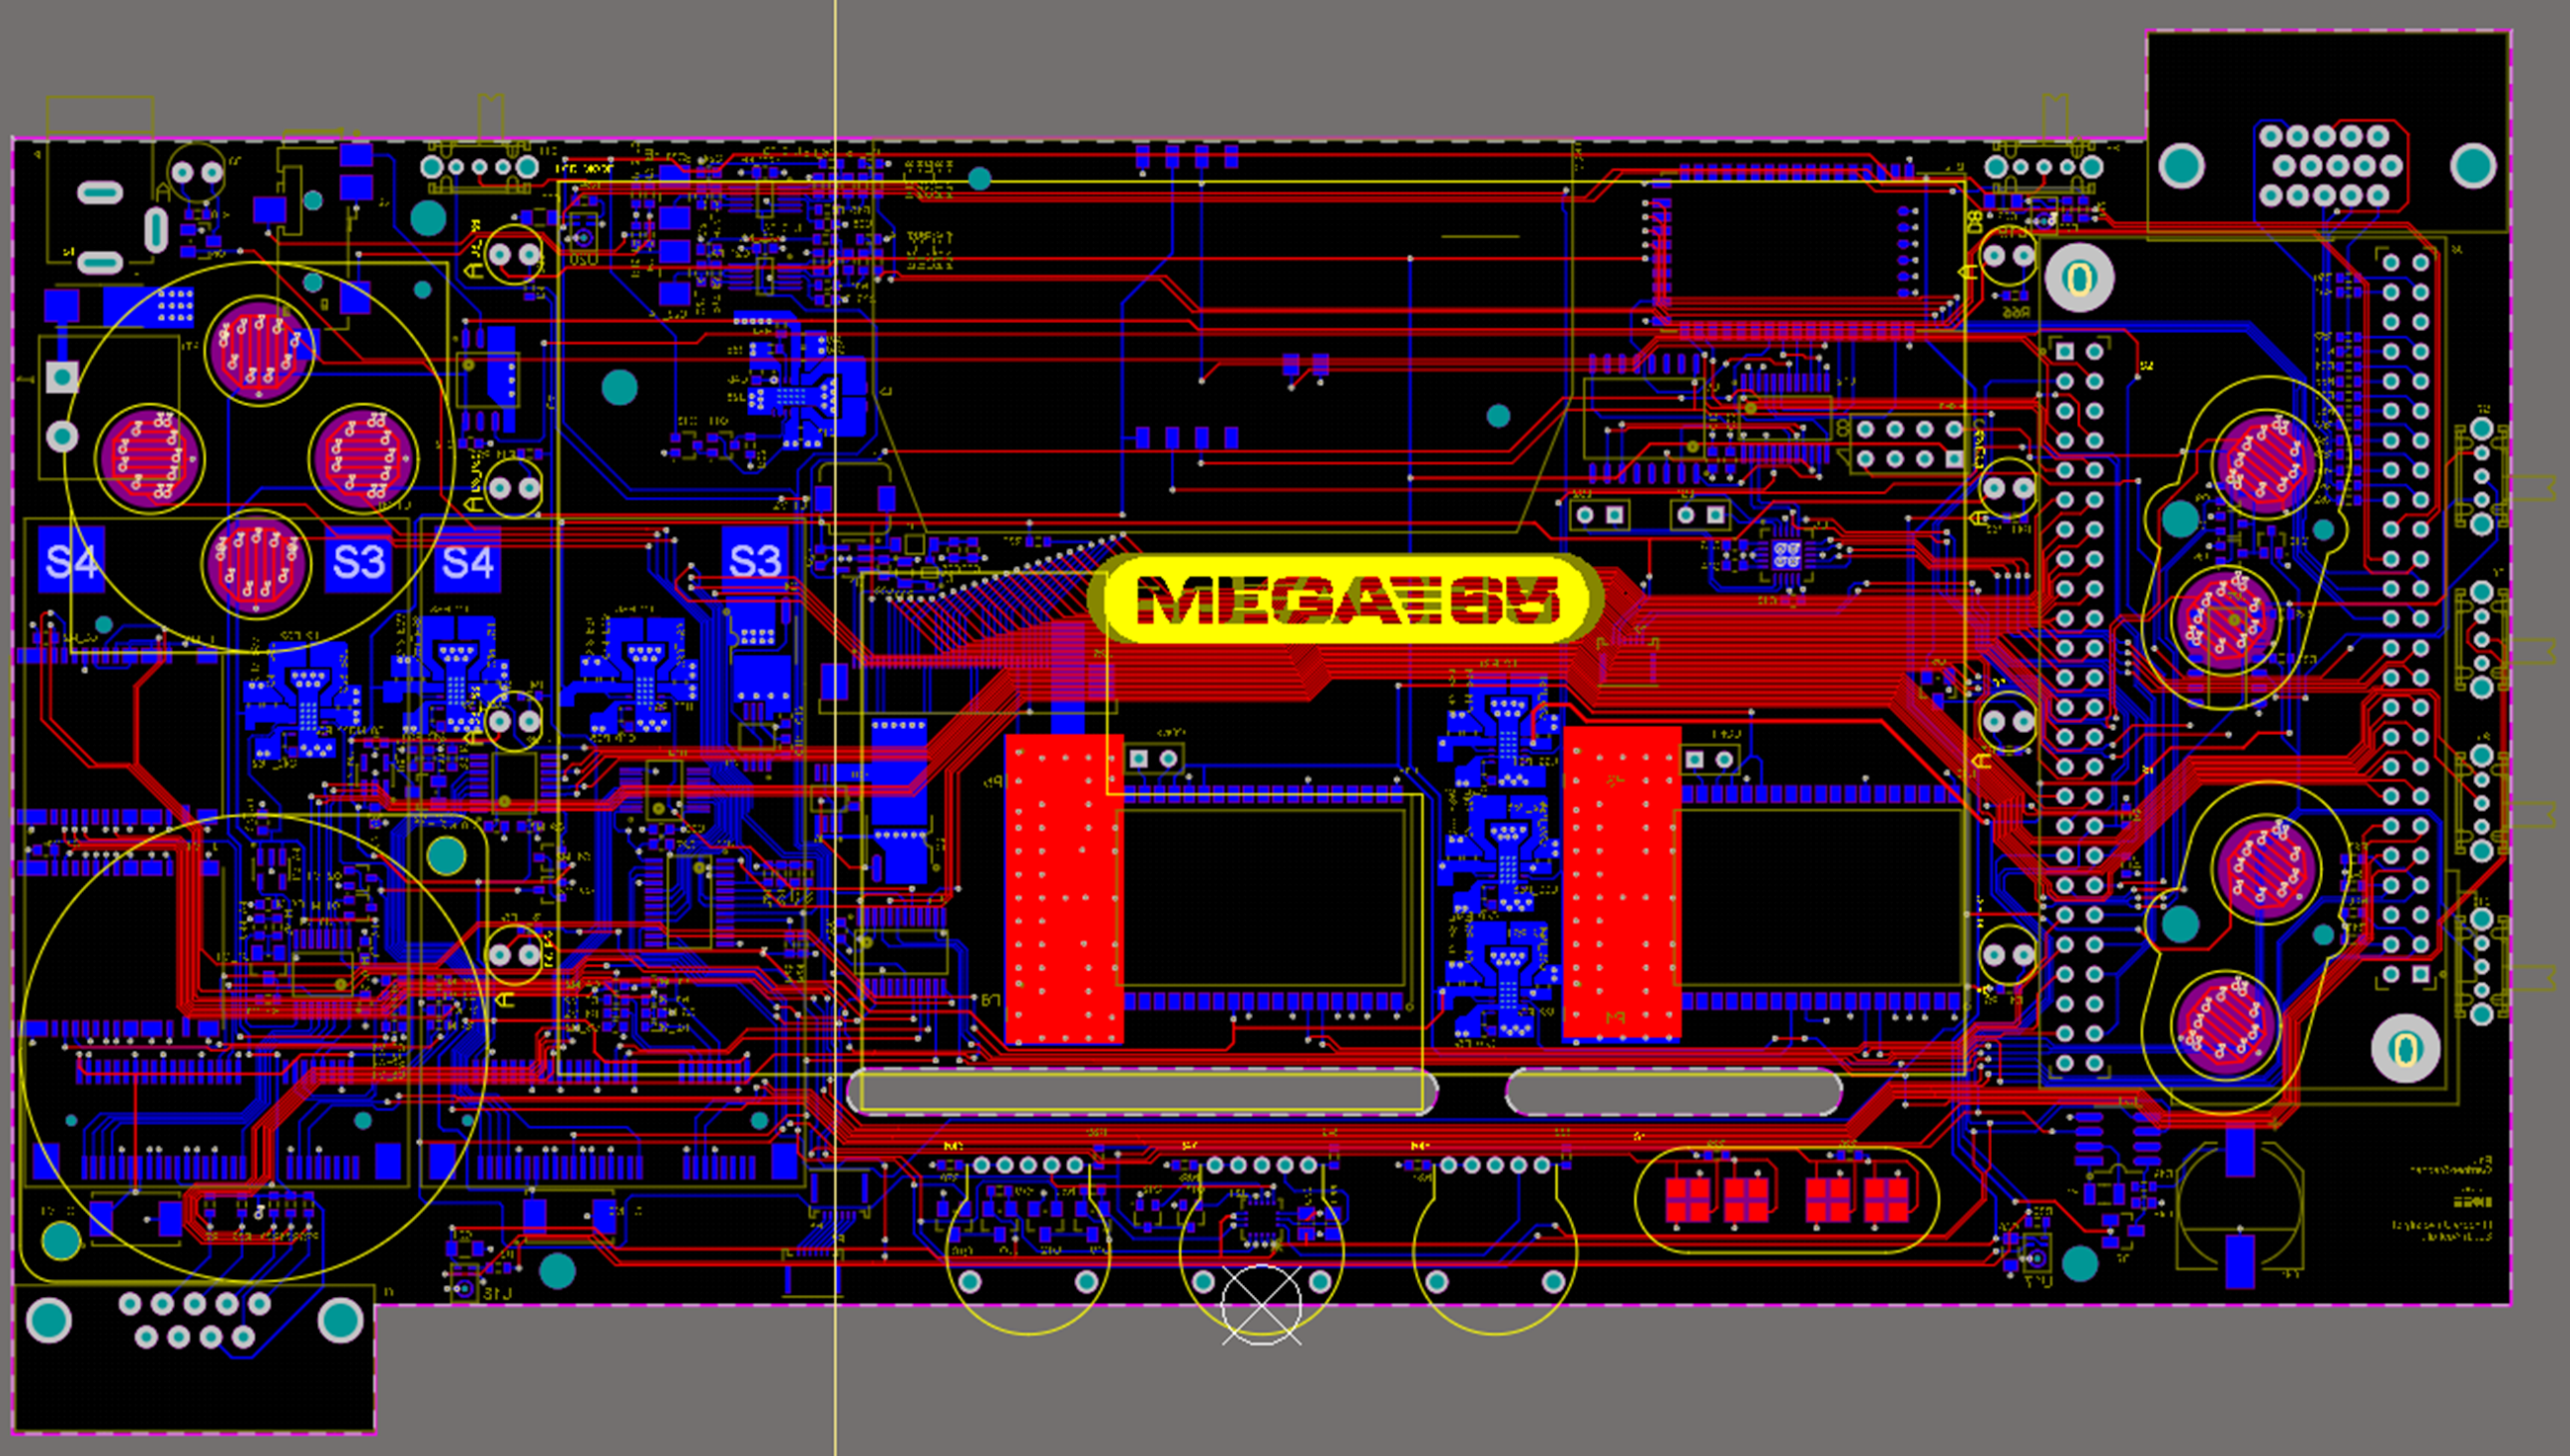
\includegraphics[width=10cm,height=10cm,keepaspectratio]{Figures/pcb_original.png}
\caption{This was the PCB layout during the development of this project.}
\label{fig:ThisFig}
\end{centering}
\end{figure}

%-----------------------------------
%	SUBSECTION 2
%-----------------------------------
\subsection{Proposed PCB Layout} \label{Proposed}

A possible solution to the existing PCB which does inhabit the UD principles is proposed in figure \ref{fig:FuturePCB}. 
The underlying idea with this redesign was to integrate the design all onto one PCB as doing so would remove the need for wires, therefore making the design overall ‘simpler’.
The reason for the redesign not being undertaken in this project has been discussed previously as impractical due to an issue of cost and time.

\begin{figure} [h]
\begin{centering}
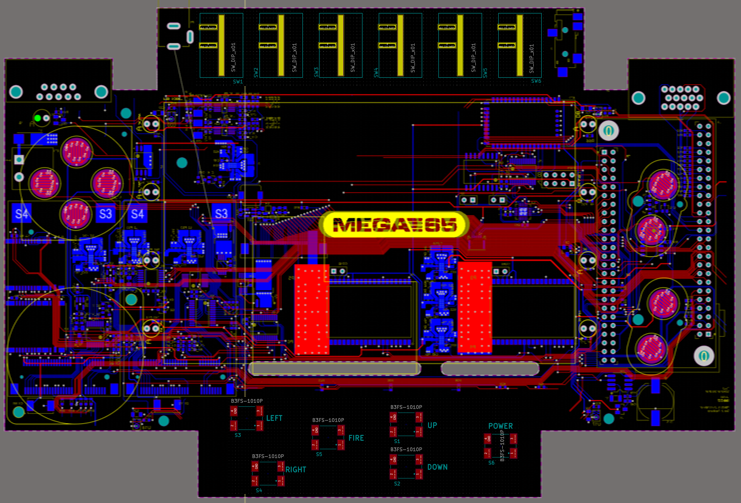
\includegraphics[width=10cm,height=10cm,keepaspectratio]{Figures/pcb_final.png}
\caption{This is the PCB as it is proposed in a future revision of the MEGAphone project.}
\label{fig:FuturePCB}
\end{centering}
\end{figure}

In order to make the device more intuitive, placement of the 9-pin DSUB port should be moved to the ‘top’ of the device in the same orientation as the VGA port, so that users know from a glance that this is where all device ports are expected to be.
The accessible button interface also utilises an external PCB which hosts the tactile switches that were opted to form the base of the accessible button function.

Other options were considered, such as silicone rubber pads, as used for the directional button and ‘A’, ‘B’ buttons. 
However, primarily due to the size, larger buttons would be recommended as this would make button presses easier for all users, ignoring the EZ keys in this scenario.
It is acknowledged that larger buttons on the PCB would invalidate the current Gameboy buttons, which is why a complete redesign of those buttons would be recommended to further progress the accessibility of the device as a whole.

It is also recommended that the PCB incorporates multiple 3.5mm jack inputs, separate from the audio function, in its design as this can give users the ability to plug in multiple switches much like the Jellybean presented in this project (view chapter \ref{Jellybean Switch}).
Microsoft's accessible controller \cite{adaptive} is a prime example of the usefulness of this feature and for those who might not be able to interact with the EZ keys or Gameboy buttons but desire their means of interaction with the device, multiple inputs allow for multiple unique functions.
Placement of these inputs should theoretically be at the 'top' of the device with all other ports, as this minimises complexity by ensuring that everything is in one place for the user.

%-----------------------------------
%	SUBSECTION 3
%-----------------------------------
\subsection{MEGAphone Housing} \label{FutureHousing}

There are a few recommendations regarding the design of the housing for the MEGAphone project.
The space around the power and audio ports of the device could benefit from being better filled in around further working toward a better-sealed device.

The handgrip aspect of the device could also benefit from some refinement.
Although physical use with the device was comfortable, it was observed that the hand-grip did not do enough to support the user's thumbs (view chapter \ref{Handgrip}).
While the ridges on the 'top' housing fit their purpose in guiding the user's hands to the correct place, they are less important than the ridges at the 'bottom' of the device.
Therefore, more focus on support for how the user's thumbs rest on top of the device would benefit this project far more.

\begin{figure} [h]
    \centering
    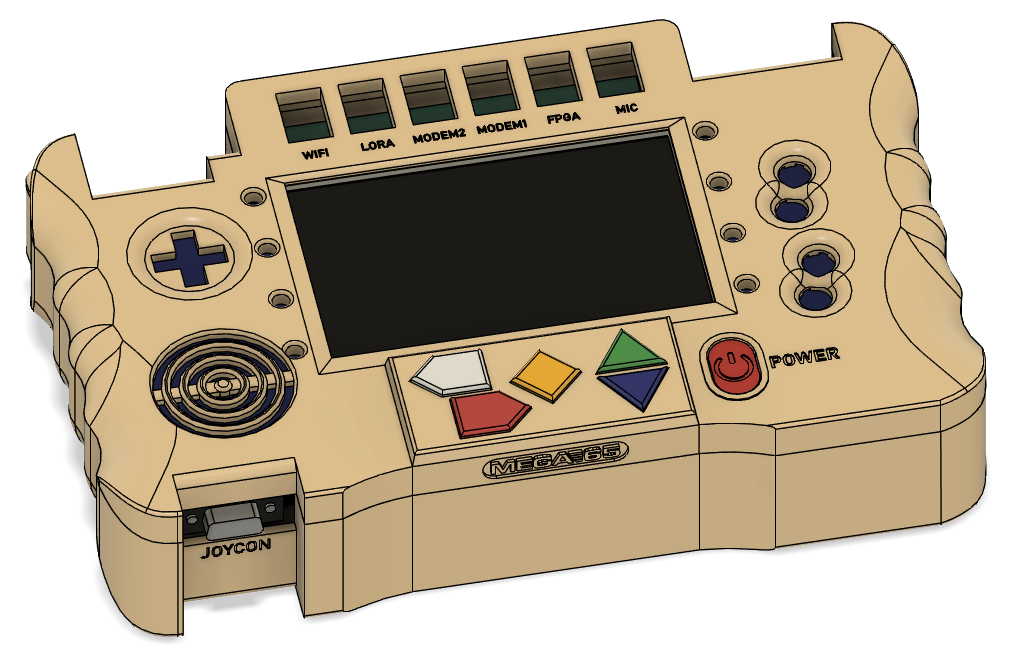
\includegraphics[width=10cm,height=10cm,keepaspectratio]{Figures/final_front_cad.png}
    \caption{This is the final top view of the device, where the 'EZ access' keys and power button can be seen nicely colour coded.}
    \label{fig:FinalTOP}
\end{figure}

An effective solution to the water-resistant ventilation problem brought up in chapter \ref{Vents} might be to explore a tightly integrated mesh, similar to what might be found on modern in-ear headphones.
This should repel water droplets to some degree or at least limit the ease in which water can enter the device.
It is worth noting that, as mentioned previously, thermal management is a very low priority given the low-power operation of the device.

As previously mentioned, a better interlocking mechanism for the updated solar panel feature would benefit the usability of the device when inserting or removing solar cells.

\begin{figure} [h]
    \centering
    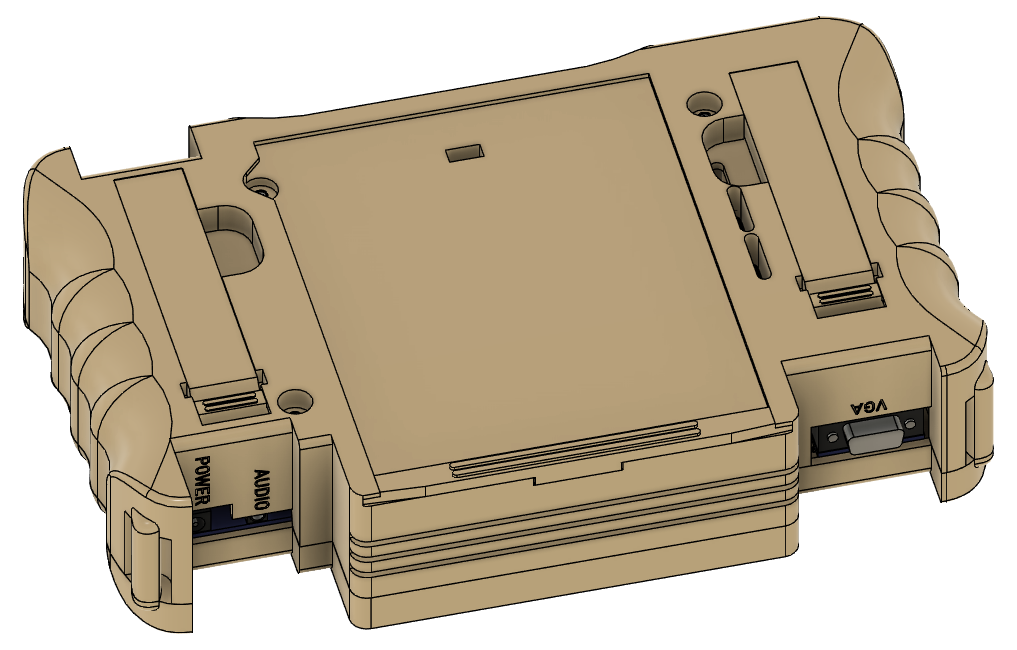
\includegraphics[width=10cm,height=10cm,keepaspectratio]{Figures/final_back_cad.png}
    \caption{This is the final bottom view, where the updated solar panel housing and accessible 'stands' can be seen.}
    \label{fig:FinalBOTTOM}
\end{figure}

Additionally, a more refined method of extending out the two device stands would be useful, accompanied by a locking feature for quality of life.
While the current implementation does 'lock' the stand in place to some degree, however, if the device is tilted upside down, this 'locking' mechanism will likely fail.
As well as this, it is suggested that a future iteration attempts the alternative method (view chapter \ref{Stand}) of mounting the stand to the cylindrical housing as the current design presented some structural weakness when testing the physical prototype.

Ultimately, emphasis should be placed on redesigning the MEGAphone PCB first and foremost (in section \ref{Proposed}).

%-----------------------------------
%	SUBSECTION 4
%-----------------------------------
\subsection{MEGA65 Accessibility}

This project introduced a new method of interacting with the on-screen keyboard via a Jellybean switch (view chapter \ref{Jellybean Switch} and chapter \ref{Software Access}).
Future studies into this space could look into more accessibility features within the MEGA65 OS, such as contrast and colour features for the visually impaired, including colour blindness.
As well as this, an array of multiple Jellybean switches (or other digital input switches) could look at emulating the actions of a joystick controller.
Much in the spirit of Microsoft's accessible controller, the MEGAphone could provide an accessible controller for fans of retro Commodore64 games.

%----------------------------------------------------------------------------------------
%	SECTION 4
%----------------------------------------------------------------------------------------

\section{Final Product}
The final product as a result of the development discussed in chapter \ref{Chapter4} and changes made in chapter \ref{Chapter5} is presented.
It can be observed from figure \ref{fig:FinalTOP} and figure \ref{fig:FinalBOTTOM} that the final colour scheme is shown, as it is intended.
This differs from the 3D-printed prototypes which were unglamorous in comparison as they were printed with white PLA plastic.
However, for testing, this was unproblematic.

Assets for this project will remain in Dr Paul Gardner-Stephen's possession in the event of future work on this project.
Eventually, it is the intention that those assets are provided to MEGAphone users, to support their right to modify design aspects to suit their needs.

%----------------------------------------------------------------------------------------
%	SECTION 5
%----------------------------------------------------------------------------------------

\section{Final Summary}
This final concluding chapter recalls the research questions and contributions of the author originally discussed in the first chapter.
Those research questions and contributions were listed in this chapter and provided with short summaries as to how each item was addressed in this thesis, supported by evidence.
Future development towards this project was discussed, where suggestions on what should be addressed next were provided, with explanations as to why each aspect should be approached in a particular way.

This project deliverable has provided the MEGAphone with a substantial platform in which to conduct future studies into UD.
An investigation into the importance of UD and DS and how they can work together to provide a platform for otherwise marginalised groups was well conducted.
As can be seen, by the outcome of the main deliverable, this project is a testament to designing for accessibility and how it allows anyone to enjoy the benefits that the MEGAphone has to offer arguably to a much greater degree than before.
As well as supporting people with a disability or old age, designing for accessibility also enhances the useability for those who are perfectly able-bodied, which has lead to a more well-refined device overall.